% Options for packages loaded elsewhere
\PassOptionsToPackage{unicode}{hyperref}
\PassOptionsToPackage{hyphens}{url}
\PassOptionsToPackage{dvipsnames,svgnames,x11names}{xcolor}
%
\documentclass[
  letterpaper,
  DIV=11,
  numbers=noendperiod]{scrartcl}

\usepackage{amsmath,amssymb}
\usepackage{lmodern}
\usepackage{iftex}
\ifPDFTeX
  \usepackage[T1]{fontenc}
  \usepackage[utf8]{inputenc}
  \usepackage{textcomp} % provide euro and other symbols
\else % if luatex or xetex
  \usepackage{unicode-math}
  \defaultfontfeatures{Scale=MatchLowercase}
  \defaultfontfeatures[\rmfamily]{Ligatures=TeX,Scale=1}
\fi
% Use upquote if available, for straight quotes in verbatim environments
\IfFileExists{upquote.sty}{\usepackage{upquote}}{}
\IfFileExists{microtype.sty}{% use microtype if available
  \usepackage[]{microtype}
  \UseMicrotypeSet[protrusion]{basicmath} % disable protrusion for tt fonts
}{}
\makeatletter
\@ifundefined{KOMAClassName}{% if non-KOMA class
  \IfFileExists{parskip.sty}{%
    \usepackage{parskip}
  }{% else
    \setlength{\parindent}{0pt}
    \setlength{\parskip}{6pt plus 2pt minus 1pt}}
}{% if KOMA class
  \KOMAoptions{parskip=half}}
\makeatother
\usepackage{xcolor}
\setlength{\emergencystretch}{3em} % prevent overfull lines
\setcounter{secnumdepth}{5}
% Make \paragraph and \subparagraph free-standing
\ifx\paragraph\undefined\else
  \let\oldparagraph\paragraph
  \renewcommand{\paragraph}[1]{\oldparagraph{#1}\mbox{}}
\fi
\ifx\subparagraph\undefined\else
  \let\oldsubparagraph\subparagraph
  \renewcommand{\subparagraph}[1]{\oldsubparagraph{#1}\mbox{}}
\fi


\providecommand{\tightlist}{%
  \setlength{\itemsep}{0pt}\setlength{\parskip}{0pt}}\usepackage{longtable,booktabs,array}
\usepackage{calc} % for calculating minipage widths
% Correct order of tables after \paragraph or \subparagraph
\usepackage{etoolbox}
\makeatletter
\patchcmd\longtable{\par}{\if@noskipsec\mbox{}\fi\par}{}{}
\makeatother
% Allow footnotes in longtable head/foot
\IfFileExists{footnotehyper.sty}{\usepackage{footnotehyper}}{\usepackage{footnote}}
\makesavenoteenv{longtable}
\usepackage{graphicx}
\makeatletter
\def\maxwidth{\ifdim\Gin@nat@width>\linewidth\linewidth\else\Gin@nat@width\fi}
\def\maxheight{\ifdim\Gin@nat@height>\textheight\textheight\else\Gin@nat@height\fi}
\makeatother
% Scale images if necessary, so that they will not overflow the page
% margins by default, and it is still possible to overwrite the defaults
% using explicit options in \includegraphics[width, height, ...]{}
\setkeys{Gin}{width=\maxwidth,height=\maxheight,keepaspectratio}
% Set default figure placement to htbp
\makeatletter
\def\fps@figure{htbp}
\makeatother
\newlength{\cslhangindent}
\setlength{\cslhangindent}{1.5em}
\newlength{\csllabelwidth}
\setlength{\csllabelwidth}{3em}
\newlength{\cslentryspacingunit} % times entry-spacing
\setlength{\cslentryspacingunit}{\parskip}
\newenvironment{CSLReferences}[2] % #1 hanging-ident, #2 entry spacing
 {% don't indent paragraphs
  \setlength{\parindent}{0pt}
  % turn on hanging indent if param 1 is 1
  \ifodd #1
  \let\oldpar\par
  \def\par{\hangindent=\cslhangindent\oldpar}
  \fi
  % set entry spacing
  \setlength{\parskip}{#2\cslentryspacingunit}
 }%
 {}
\usepackage{calc}
\newcommand{\CSLBlock}[1]{#1\hfill\break}
\newcommand{\CSLLeftMargin}[1]{\parbox[t]{\csllabelwidth}{#1}}
\newcommand{\CSLRightInline}[1]{\parbox[t]{\linewidth - \csllabelwidth}{#1}\break}
\newcommand{\CSLIndent}[1]{\hspace{\cslhangindent}#1}

\usepackage{booktabs}
\usepackage{longtable}
\usepackage{array}
\usepackage{multirow}
\usepackage{wrapfig}
\usepackage{float}
\usepackage{colortbl}
\usepackage{pdflscape}
\usepackage{tabu}
\usepackage{threeparttable}
\usepackage{threeparttablex}
\usepackage[normalem]{ulem}
\usepackage{makecell}
\usepackage{xcolor}
\KOMAoption{captions}{tableheading}
\makeatletter
\makeatother
\makeatletter
\makeatother
\makeatletter
\@ifpackageloaded{caption}{}{\usepackage{caption}}
\AtBeginDocument{%
\ifdefined\contentsname
  \renewcommand*\contentsname{Table of contents}
\else
  \newcommand\contentsname{Table of contents}
\fi
\ifdefined\listfigurename
  \renewcommand*\listfigurename{List of Figures}
\else
  \newcommand\listfigurename{List of Figures}
\fi
\ifdefined\listtablename
  \renewcommand*\listtablename{List of Tables}
\else
  \newcommand\listtablename{List of Tables}
\fi
\ifdefined\figurename
  \renewcommand*\figurename{Figure}
\else
  \newcommand\figurename{Figure}
\fi
\ifdefined\tablename
  \renewcommand*\tablename{Table}
\else
  \newcommand\tablename{Table}
\fi
}
\@ifpackageloaded{float}{}{\usepackage{float}}
\floatstyle{ruled}
\@ifundefined{c@chapter}{\newfloat{codelisting}{h}{lop}}{\newfloat{codelisting}{h}{lop}[chapter]}
\floatname{codelisting}{Listing}
\newcommand*\listoflistings{\listof{codelisting}{List of Listings}}
\makeatother
\makeatletter
\@ifpackageloaded{caption}{}{\usepackage{caption}}
\@ifpackageloaded{subcaption}{}{\usepackage{subcaption}}
\makeatother
\makeatletter
\@ifpackageloaded{tcolorbox}{}{\usepackage[many]{tcolorbox}}
\makeatother
\makeatletter
\@ifundefined{shadecolor}{\definecolor{shadecolor}{rgb}{.97, .97, .97}}
\makeatother
\makeatletter
\makeatother
\ifLuaTeX
  \usepackage{selnolig}  % disable illegal ligatures
\fi
\IfFileExists{bookmark.sty}{\usepackage{bookmark}}{\usepackage{hyperref}}
\IfFileExists{xurl.sty}{\usepackage{xurl}}{} % add URL line breaks if available
\urlstyle{same} % disable monospaced font for URLs
\hypersetup{
  pdftitle={Digitization of the Australian Parliamentary Debates, 1998-2022},
  pdfauthor={Lindsay Katz; Rohan Alexander},
  colorlinks=true,
  linkcolor={blue},
  filecolor={Maroon},
  citecolor={Blue},
  urlcolor={Blue},
  pdfcreator={LaTeX via pandoc}}

\title{Digitization of the Australian Parliamentary Debates, 1998-2022}
\author{Lindsay Katz\footnote{University of Toronto,
  lindsay.katz@mail.utoronto.ca} \and Rohan Alexander\footnote{University
  of Toronto, rohan.alexander@utoronto.ca}}
\date{January 20, 2023}

\begin{document}
\maketitle
\begin{abstract}
Public knowledge of what is said in parliament is a key tenet of
democracy, and a critical resource for political science research. In
Australia, following the British tradition, the written record of what
is said in parliament is known as Hansard. While the Australian Hansard
has always been publicly available, it has been difficult to use it for
the purpose of large-scale macro and micro-level text analysis because
it has not been available as a dataset of sufficient quality. Following
the lead of the Linked Parliamentary Data project which achieved this
for Canada, we provide a new, comprehensive, high-quality database that
captures all proceedings of the Australian parliamentary debates from
1998 to the present using Hansard. The database is publicly available
and can be readily linked to other datasets such as election results.
The creation and accessibility of this database will enable the
exploration of questions that are not currently possible to explore,
serving as a valuable resource for both researchers and policymakers.
\end{abstract}
\ifdefined\Shaded\renewenvironment{Shaded}{\begin{tcolorbox}[enhanced, breakable, borderline west={3pt}{0pt}{shadecolor}, sharp corners, interior hidden, boxrule=0pt, frame hidden]}{\end{tcolorbox}}\fi

\hypertarget{sec-intro}{%
\section{Background \& Summary}\label{sec-intro}}

The official written record of parliamentary debates, formally known as
Hansard, plays a fundamental role in capturing the history of political
proceedings and facilitating the exploration of valuable research
questions. Originating in the British parliament, the production of
Hansard became tradition in a number of Commonwealth countries such as
Canada, the United Kingdom, and Australia (Vice and Farrell 2017). Given
the content and magnitude of these records, they have significance,
particularly in the context of political science research. In the case
of Canada, a team of researchers at the University of Toronto have
digitized Hansard from 1901 to 2019, an endeavour called the Linked
Parliamentary Data (LiPaD) project (Beelen et al. 2017). Having a
digitized version of Hansard enables researchers to perform advanced
analyses on these records using text analysis tools and statistical
modelling. Following the lead of the LiPaD project, in this paper we
introduce a novel database for the Australian Hansard. This is composed
of individual datasets for each sitting day in the House of
Representatives from 1998 to 2022, containing details on everything said
in parliament in a form which can be readily used by researchers. With
the development of tools for large-scale text analysis, this database
will serve as a valuable resource for efficiently studying and exploring
political behaviour in Australia over time.

The House of Representatives performs a number of crucial governmental
functions, such as creating new laws and overseeing government
expenditure (House of Representatives 2018, ch.~1). The House operates
under a parallel chamber setup, meaning there are two debate venues
where proceedings take place: the Chamber, and the Federation Chamber.
Sittings of the House follow a predefined order of business, regulated
by procedural rules called standing orders (House of Representatives
2018, ch.~8). A typical sitting day in the Chamber has a number of
scheduled proceedings including debates on government business, 90
second member statements, and Question Time (House of Representatives
2018, ch.~8). The Federation Chamber was created in 1994 as a
subordinate debate venue of the Chamber. This allows for better time
management of House business as its proceedings occur simultaneously
with those of the Chamber (House of Representatives 2018, ch.~21).
Sittings in the Federation Chamber are quite different to those of the
Chamber in terms of their order of business and scope of discussion.
Business matters discussed in the Federation Chamber are limited largely
to intermediate stages of bill development, and the business of private
Members (House of Representatives 2018, ch.~21). It is the recording and
compilation of all of these proceedings on which Hansard is based, and
it is essentially, but not entirely, verbatim.

A week or so after each sitting day, a transcript is available for
download from the official Parliament of Australia website in both
static PDF and extensible markup language (XML) form. The PDF is the
official release, which is converted to typed text using Optical
Character Recognition (OCR) technology (Sherratt 2016). This conversion
allows for the production of the XML formatted transcript, though these
are not always perfect conversions and are particularly flawed in the
early decades of Hansard (Sherratt 2016). The PDF imposes formatting
designed for humans to read with ease, whereas XML is designed for
consistency and machine legibility. The nature of XML enables us to more
easily use code to manipulate these records at scale, motivating our
choice to develop our database solely using the XML formatted files. In
cases where we were unsure on how to proceed with processing the XML, we
defer first to the PDF, and then to the video recording of the
proceeding if available.

At present, the Hansard format that is available on the Parliament of
Australia website is not accessible for large scale analysis. To this
point, various researchers have had to create their own databases in an
attempt to produce usable, complete data based on content from the
Australian Parliament website. For instance, Sherratt (2016) created an
online, easy to read database of Hansard from 1901 to 1980 using the XML
files. These data can be navigated by year, parliament, people, and
bills (Sherratt 2016). In an effort to make the Australian Parliamentary
Handbook more accessible, Leslie (2021) has released an \texttt{R}
package which includes data on all Members of the Australian House of
Representatives from 1945 to 2019. Further, Alexander and Hodgetts
(2021) created the \texttt{AustralianPoliticians} \texttt{R} package,
which contains a number of datasets related to the political and
biographical information of Australian federal politicians who were
active between 1901 and 2021.

A number of papers exist which utilize components of Australian Hansard
to explore various research topics. For example, Salisbury (2011) used
online Hansard records to investigate the occurrences of unparliamentary
comments by members of the House, where The Speaker tells that member to
withdraw their remark. Rasiah (2010) worked with Question Time data from
Hansard transcripts during February and March of 2003, to investigate
resistance of politicians in answering questions about Iraq. In their
work, Fraussen, Graham, and Halpin (2018) use Hansard to quantify
political prominence by investigating strategic mentions of interest
groups by elected officials. Finally, the work of Alexander and
Alexander (2021) offers a dataset of the Australian Hansard, along with
an analysis of the effect of elections and changes in Prime Ministers
upon topics mentioned in parliament. Alexander and Alexander (2021)
created this database with the static PDF versions of Hansard, using OCR
to digitize these files into text which is suitable for analysis. This
means there are considerable digitization errors especially in the first
half of the dataset.

While there is evidently a growing body of literature on this topic,
there is still no comprehensive database for Australian Hansard based on
XML that spans from 1901 to the present day. Our work serves to bridge
this gap.

\hypertarget{methods}{%
\section{Methods}\label{methods}}

Our database contains one comma-separated value (CSV) file for each
sitting day of the House of Representatives from 02 March 1998 to 08
September 2022. We developed four scripts to produce all of these files,
where each script is designed to parse Hansard documents from a specific
portion of the 1998 to 2022 time frame.

This section will be structured as follows. First, we will provide an
overview of our approach to understanding and parsing an individual
Hansard XML document, which informed all four scripts used to create our
database. This will be supplemented with an excerpt from a Hansard XML
to provide a visual example of its structure. Next we will explain the
specific differences between the four scripts, and outline what
structural changes necessitated their separate development. We will then
provide details on the methodological intricacies of three core
components of Hansard proceedings: Question Time, interjections, and
stage directions.

\hypertarget{sec-overview}{%
\subsection{Overview}\label{sec-overview}}

The approach to parsing contents of an XML document is heavily dependent
on its tree structure. As such, to create this database, we started by
looking at a single Hansard XML transcript from 2019. Doing so enabled
us to identify the various components of interest in the document, and
how each one can be parsed according to its corresponding structural
form. Parsing was performed in \texttt{R} using the \texttt{XML} and
\texttt{xml2} packages (Temple Lang 2022; Wickham, Hester, and Ooms
2021). Focusing on one transcript also allowed us to ensure that all key
components of the transcript were being parsed and captured with as much
detail as possible. The typical form of a Hansard XML transcript is
summarized in the nested list below. Note that this provides a broad
overview of the structure, and does not contain every possible nested
element that may be found in a Hansard XML.

\begin{quote}
\begin{verbatim}
     <hansard>
       1. <session.header>
       2. <chamber.xscript>
          a)  <business.start>
          b)  <debate>
              i.  <debateinfo>
              ii. <debate.text>
              iii. <speech>
              iv. <subdebate.1>
                  (1) <subdebateinfo>
                  (2) <subdebate.text>
                  (3) <speech>
                  (4) <subdebate.2>
                      (a) <subdebateinfo>
                      (b) <subdebate.text>
                      (c) <speech>
      3. <fedchamb.xscript>
      4. <answers.to.questions>
          a)  <question>
          b)  <answer>
\end{verbatim}
\end{quote}

The outer-most node, also known as the parent node, is denoted
\texttt{\textless{}hansard\textgreater{}} and serves as a container for
the entire document. This parent node may have up to four child-nodes,
where the first child-node contains details on the specific sitting day.
Next, \texttt{\textless{}chamber.xscript\textgreater{}} contains all
proceedings of the Chamber,
\texttt{\textless{}fedchamb.xscript\textgreater{}} contains all
proceedings of the Federation Chamber, and
\texttt{\textless{}answers.to.questions\textgreater{}} contains Question
Time proceedings. Note that the Federation Chamber does not meet on
every sitting day, so this child element is not present in every XML
file. The use of separate child nodes allows for the distinction of
proceedings of the Chamber and Federation Chamber. The structure of the
\texttt{\textless{}chamber.xscript\textgreater{}} and
\texttt{\textless{}fedchamb.xscript\textgreater{}} nodes are generally
the same, where the proceeding begins with a business start which is
followed by a series of debates. Debate nodes can contain a sub-debate 1
child-node which has a sub-debate 2 child-node nested within it. That
said, sometimes sub-debate 2 is not nested within sub-debate 1. Each of
these three elements (i.e.~\texttt{\textless{}debate\textgreater{}},
\texttt{\textless{}subdebate.1\textgreater{}}, and
\texttt{\textless{}subdebate.2\textgreater{}}) as well as their
respective sub-elements contain important information on the topic of
discussion, who is speaking, and what is being said. The
\texttt{\textless{}speech\textgreater{}} node within each one contains
the bulk of the text associated with that debate or sub-debate. A
typical \texttt{\textless{}speech\textgreater{}} node begins with a
\texttt{\textless{}talk.start\textgreater{}} sub-node, providing
information on the speaker and the time of their first statement.
Unsurprisingly, speeches rarely go uninterrupted in parliamentary debate
settings --- they are often composed of a series of interjections and
continuations. These statements are categorized under different
sub-nodes depending on their nature, such as
\texttt{\textless{}interjection\textgreater{}} or
\texttt{\textless{}continuation\textgreater{}}. The final key component
of Hansard is Question Time, in which questions and answers are
classified as unique elements. More detail on the purpose and processing
of Question Time will follow in Section~\ref{sec-qa}.

Figure~\ref{fig-xml1} provides an example of the beginning of an XML
file for Hansard, which illustrates the structure outlined in the nested
list above. As stated, the XML structure begins with a parent element
\texttt{"hansard"} (highlighted in blue), followed by a child element
\texttt{"session.header"} (highlighted in yellow) with sub-child
elements such as the date and parliament number, which are all
highlighted in pink. Next there is the child element containing
everything that takes place in the Chamber, \texttt{"chamber.xscript"},
which is also highlighted in yellow in Figure~\ref{fig-xml1}. As
previously mentioned, the first sub-node of \texttt{"chamber.xscript"}
is the business start. The structure of the business start can be seen
between the nodes highlighted in green in Figure~\ref{fig-xml1}, where
the content we parse from the business start are highlighted in orange.

\textbf{does this feel a bit repetitive? do you think it's worth
keeping?}

\begin{figure}

{\centering 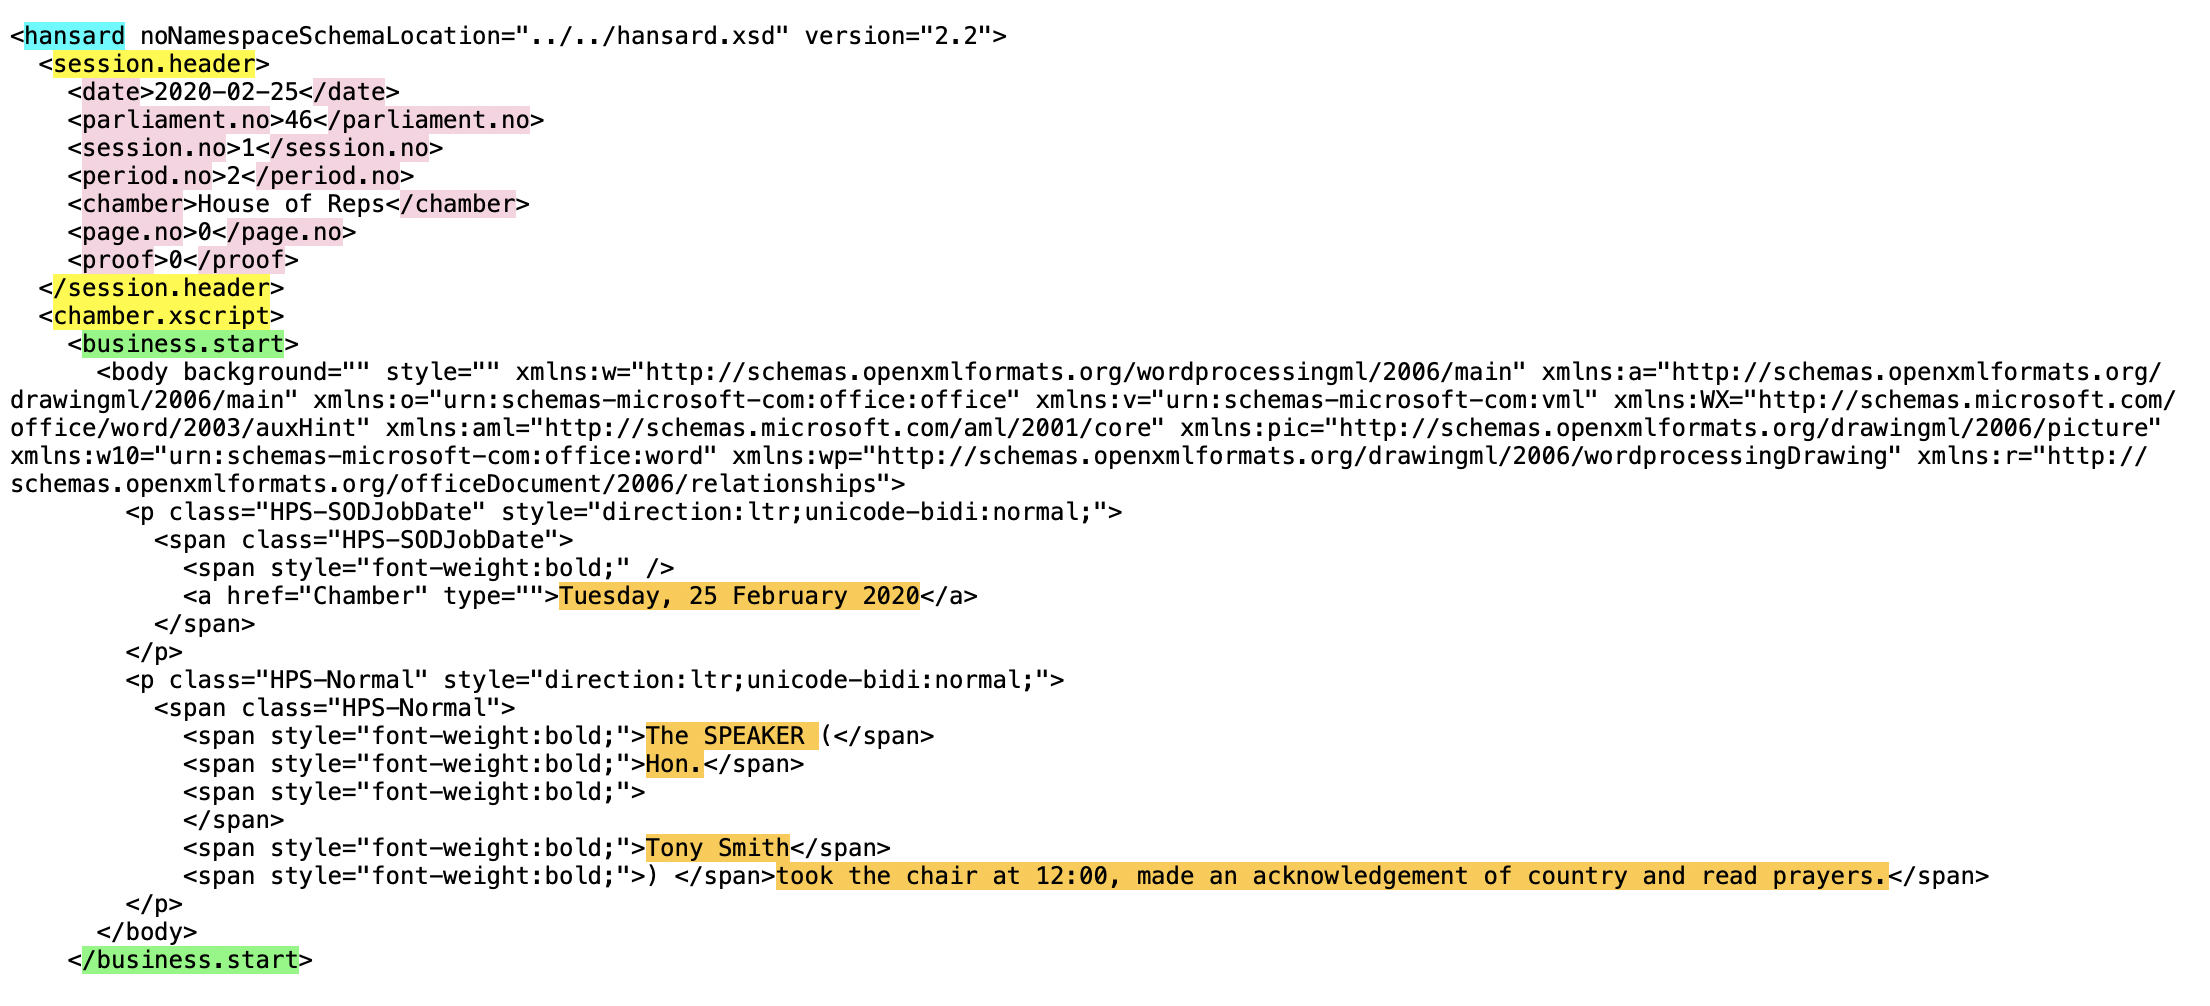
\includegraphics{xml1.png}

}

\caption{\label{fig-xml1}Snapshot of beginning of XML file for Hansard
on 25 February 2020}

\end{figure}

Evidently, the nature of XML formatting means that different pieces of
information are categorized under a series of uniquely named and nested
nodes. As a result, to parse each piece of information, one must specify
the unique hierarchy of nodes in which it is structured. This is known
as an XPath expression, and tells the parser how to navigate the XML
document to obtain the desired information. For example, the session
header date in Figure~\ref{fig-xml1} can be accessed using the XPath
expression ``\texttt{hansard/session.header/date}''. We began our first
script by parsing every piece of information contained in the XML
document, using these unique XPath expressions to do so.

The next step was to further develop our script to produce tidy data
sets containing each parsed element, where each statement is separated
onto its own row with details about the speaker, and rows are placed in
chronological order. This first involved correcting the variable classes
and adding a number of indicator variables to differentiate where
statements came from, such as Chamber versus Federation Chamber or
sub-debate 1 versus sub-debate 2. The next key task stemmed from the
fact that the raw text data were not separated by each statement when
parsed. In other words, any interjections, comments made by The Speaker
or Deputy Speaker and continuations within an individual speech were all
parsed together as a single string. As such, the name, name ID,
electorate and party details were only provided for the person whose
turn it was to speak. Splitting up these speeches in a way which would
be generalizable across sitting days required much thought and effort.
Section~\ref{sec-interject} will provide further details on the
intricacies of this task.

Since we are looking at a wide time span of documents, there are
expectedly a number of changes in the way they are formatted over time.
These became apparent as we ran our script on XML files from earlier
sitting days. Some changes are as subtle as a differently named
child-node, while others are as extensive as a completely different
nesting structure. Smaller changes were accounted for as we became aware
of them, and embedded into the code in a way that would not cause issues
for parsing more current Hansards with subtle differences in formatting.
However, as mentioned, more significant changes in the XML structure of
Hansard are what necessitated the development of separate scripts as we
worked backwards in time. Further, while working backward in time, it
became clear that not every sitting day contains every possible XML
element. For example, some days did not have sub-debate 2 content, and
some days did not have a Federation Chamber proceeding. To improve the
generalizability of these scripts, if-else statements were embedded
within the code wherever an error might arise due to a missing element.
For example, the entire Federation Chamber block of code is wrapped in
an if-else statement for each script, so that it only executes if what
the code attempts to parse actually exists in the file.

Once the script ran without error for a few recent years of Hansard, we
continued to work backwards until extensive changes in tree structure
made our script incompatible with parsing earlier XML files. The
earliest sitting day our first script can successfully parse is 14
August 2012. Before developing new scripts to parse earlier Hansard
documents, we decided to prioritize cleaning and finalizing what we have
been able to parse. As such we continued building our script, fixing any
problems we noticed in the resulting datasets such as excess whitespace
or spacing issues, and splitting up any additional sections of the
parsed text onto separate rows where necessary. Specifically, we added a
section of our script to separate out general stage directions. More
information on this separation will be provided in
Section~\ref{sec-stage}. After completing our first script, it was
formatted as a function which takes a single file name argument and
produces one CSV file containing data on all proceedings from the given
sitting day.

\hypertarget{sec-diff}{%
\subsection{Script Differences}\label{sec-diff}}

As previously mentioned, we developed a total of four scripts to parse
the 1998-2022 time frame of Hansard documents. Two main factors
motivated us to create four scripts as opposed to just one, the first
being structural variation in XML over time, and the second being
improved computational efficiency with separate scripts. While all four
scripts use the same general approach to parsing described in
Section~\ref{sec-overview} and produce the same CSV structure, the first
and second scripts use a different method of data processing than the
third and fourth scripts.

The need for a second script stems from the fact that when established
in 1994, the Federation Chamber was originally named the Main Committee.
The Main Committee was renamed to the Federation Chamber in mid-2012
(House of Representatives 2018, ch.~21). As a result, the child-node
under which Federation Chamber proceedings are nested is named
\texttt{\textless{}maincomm.xscript\textgreater{}} in all XML files
prior to 14 August 2012. Having developed our first script based on
Hansard from recent years, all XPath expressions contain the
\texttt{\textless{}fedchamb.xscript\textgreater{}} specification. To
avoid causing issues in our first script which successfully parses about
10 years of Hansard, we created a second script where we replaced all
occurrences of \texttt{\textless{}fedchamb.xscript\textgreater{}} with
\texttt{\textless{}maincomm.xscript\textgreater{}}. After making this
modification and accounting for other small changes such as time stamp
formatting, this second script successfully parses all Hansard sitting
days from 10 May 2011 to 28 June 2012 (inclusive).

While the modifications needed to develop the second script were quite
straightforward, this was not the case for our next script. The typical
tree structure of Hansard XMLs spanning from 1998 to March 2011 has an
important difference from that of XMLs released after March 2011,
necessitating many changes to be made in our methodology. In XMLs after
March 2011, which our first two scripts successfully parse, the first
two child-nodes of \texttt{\textless{}speech\textgreater{}} are
typically \texttt{\textless{}talk.start\textgreater{}}, and
\texttt{\textless{}talk.text\textgreater{}}. The first child-node
contains data on the person whose turn it is to speak, and the second
contains the entire contents of that speech --- including all
interjections, comments and continuations. After the
\texttt{\textless{}talk.text\textgreater{}} element closes, there are
typically a series of other child-nodes which provide a skeleton
structure for how the speech proceedings went in chronological order.
For example, if the speech began, was interrupted by one member, and
then continued uninterrupted until the end, there would be one
\texttt{\textless{}interjection\textgreater{}} node and one
\texttt{\textless{}continuation\textgreater{}} node following the
\texttt{\textless{}talk.text\textgreater{}} node. These would contain
details on the person who made each statement such as their party and
electorate.

In contrast, the speech contents in XMLs from 1998 up to and including
24 March 2011 are nested differently --- there is no
\texttt{\textless{}talk.text\textgreater{}} node. Rather than this
single child-node that contains all speech content, statements are
categorized in individual child-nodes. This means that unlike our code
for parsing more current Hansards, we cannot specify a single XPath
expression such as ``\texttt{debate/speech/talk.text}'' or
``\texttt{debate/subdebate.1/speech/talk.text}'' to extract all
speeches, in their entirety, at once. This difference in nesting
structure made our second script unusable for parsing transcripts
preceding 10 May 2011, and required us to change our data processing
approach considerably.

Since there are numerous speeches in a typical Hansard, each having
multiple child-nodes with the same names
(i.e.~\texttt{\textless{}continuation\textgreater{}},
\texttt{\textless{}interjection\textgreater{}}), it is difficult to
parse everything while maintaining the correct ordering of statements.
We found that the most straightforward way to preserve the ordering of
statements and to parse all speech contents at once was to parse from
the \texttt{\textless{}debate\textgreater{}} element directly. The
reason we did not use its \texttt{\textless{}speech\textgreater{}}
child-node is because every speech has a unique structure of node
children, and this makes it difficult to write code for data cleaning
which is generalizable across all speeches and sitting days.

The challenge with parsing through the
\texttt{\textless{}debate\textgreater{}} element is that every piece of
data stored in that element is parsed as a single string, including all
\texttt{\textless{}talk.start\textgreater{}} data, and all nested
sub-debate data. For example, the data shown in
Figure~\ref{fig-patternEX} would be parsed as a single string preceding
the speech content, like so:

\begin{quote}
\texttt{09:31:0010261Costello,\ Peter,\ MPMr\ COSTELLOCT4HigginsLPTreasurer10}
\end{quote}

\begin{figure}

{\centering 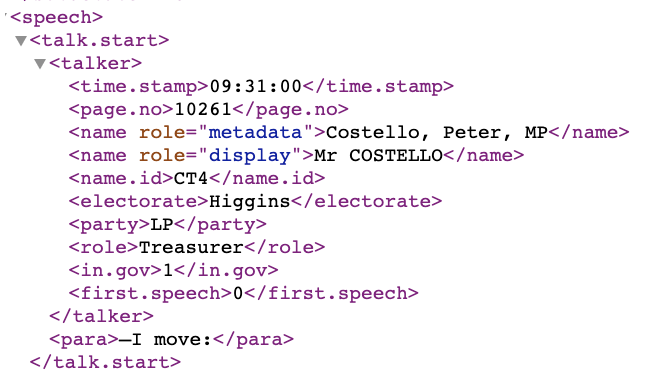
\includegraphics[width=3.28125in,height=\textheight]{patternEX.png}

}

\caption{\label{fig-patternEX}Portion of XML file for Hansard on 12
December 2002}

\end{figure}

This was not isolated to just the beginning of speeches --- details on
individuals interjecting or commenting during speeches were also
captured this way. To separate statements out correctly, we collected
all of these patterns using the
\texttt{\textless{}talk.start\textgreater{}} node, and used them to
split statements wherever one of these patterns was found. After
separating statements, we were later able remove these patterns from the
body of text. We also used this method of extracting and later removing
unwanted patterns for other pieces of data which did not belong to the
debate proceedings, such as sub-debate titles.

Once we finalized this new method of processing the data, we proceeded
with data cleaning using the same general approach as in the first two
scripts to produce the same structure of CSV output. We then worked
backwards in time and modified the code as needed for generalizability.
Throughout this process we found a number of transcription errors
present in the XMLs from earlier years. We fixed these manually,
deferring to the official release to ensure the correct information was
filled in. Since there were a number of transcription errors specific to
the 2000s, we chose to create a fourth script for parsing 1998 and 1999.
This allowed us to remove all the code which was needed to resolve
specific transcription errors of the 2000s, to avoid an overly long
script and in turn improving computational efficiency. As such, our
fourth script is essentially the same as the third, the only difference
being that it has code specific to fixing transcription errors from 1998
and 1999.

\hypertarget{sec-qa}{%
\subsection{Question Time}\label{sec-qa}}

A key characteristic of the Australian parliament system is the ability
for the executive government to be held accountable for their decisions.
One core mechanism by which this is achieved is called Question Time.
This is a period on each sitting day in the Chamber where members of the
House can ask ministers two types of questions: questions in writing
which are written in advance, or questions without notice which are
asked verbally in the Chamber and are responded to in real time (House
of Representatives 2021). Parsing the components of Question Time
required a slightly different approach than that of the debate speech,
because of its unique structure in the XML document. Questions without
notice are included directly in the \texttt{"chamber.xscript"} child
node, with sub-child nodes called \texttt{"question"} and
\texttt{"answer"} to differentiate the two. Questions in writing,
however, are embedded in their own child node called
\texttt{"answers.to.questions"} at the end of the XML file.

To parse questions without notice and questions in writing in the first
two scripts, we extracted all question and answer elements from the
\texttt{"chamber.xscript"} and \texttt{"answers.to.questions"} child
nodes. For the third and fourth scripts, our method of parsing the
\texttt{"chamber.xscript"} speeches meant that all questions without
notice content was already parsed in order. Similar to the rest of the
speech content, we used those patterns of data preceding the text to
separate questions and answers. Finally, since questions in writing
exist in their own child node we were able to use the same parsing
method for the third and fourth scripts as we did for the first and
second scripts.

We then added binary flags to differentiate between questions and
answers, determined by which sub-child node the statement was extracted
from, that is, whether it came from a
\texttt{\textless{}question\textgreater{}} node, or an
\texttt{\textless{}answer\textgreater{}} node. Sometimes, questions were
incorrectly transcribed under an answer node and vice-versa, in which
cases we manually corrected the question and answer flags using the
\texttt{str\_detect} function from the \texttt{stringr} package. For
instance, our code for parsing questions searches for any statements
which include ``has provided the following answer to the honourable
member's question'', in which case we re-code that statement as an
answer. Once all questions and answers were correctly classified as
such, we could then merge all the content back together such that each
question was followed by its associated answer. This was straightforward
due to the fact that by nature of XML parsing, all questions and answers
were parsed in the order in which they appeared in the transcript.

The next step was to merge Question Time contents with all the debate
speech. Doing so with the questions without notice content was
straightforward. For the first and second scripts, we used the time
stamp and page number associated with each question to maintain the
correct order of statements. For the third and fourth scripts, our
method of parsing meant that everything was already parsed together in
order, so we did not have to perform any additional merging. While
questions in writing do not contain time stamps, merging this content
was also straightforward due to the fact that it is always at the very
end of Hansard. This means that we could simply bind question in writing
rows to the bottom of the main dataframe. This approach was used for all
four scripts.

\hypertarget{sec-interject}{%
\subsection{Interjections}\label{sec-interject}}

As mentioned, the text was structured and parsed in such a way that
various interjections and comments which happened during a speech were
not separated onto individual rows. This was the case across the entire
time frame of documents. We will first discuss the methodology employed
to split interjections in the first and second scripts, as it informed
our approach for the third and fourth scripts.

Below is an example of part of a speech we would need to split,
extracted from Hansard on 30 November 2021, where Mr.~van Manen is
interrupted by The Speaker who states that the time for members'
statements has concluded.

\begin{quote}
``Mr VAN MANEN (Forde---Chief Government Whip) (13:59): It's a great
pleasure to share with the House that Windaroo Valley State High School
has qualified for the finals of the Australian Space Design Competition,
to begin in January next year. The competition is regarded as the
premier STEM competition for high school students and is recognised by
universities around the country. The students are required to respond to
industry-level engineering and requests for tender for design and---The
SPEAKER: Order! In accordance with standing order 43, the time for
members' statements has concluded.''
\end{quote}

We want each statement on its own row with the correct name, name ID,
electorate and party information on the individual speaking. We
approached this task in a number of steps.

Once all parsed text from the XML was merged into one dataframe called
\texttt{main}, our first step was to add a \texttt{"speech\_no"}
variable. This was done to keep track of which speech each interjection,
comment, or continuation belonged to as we separated these components
onto their own rows.

The next step was to extract all the names and titles preceding these
interjections, comments and continuations. This would enable us to then
separate the speeches in the correct places using these names and titles
in combination with regular expressions, which are patterns of
characters that can be used to search bodies of text. We completed this
extraction process with a few intermediate steps, due to the large
number of name styles and interjection types that had to be accounted
for, each requiring their own unique regular expression format.

As mentioned in Section~\ref{sec-diff}, more recent years of Hansard
XMLs contain a series of child-nodes which exist to capture the
structure of interruptions in that speech. Figure~\ref{fig-xml3}
provides an example of this, where the speech was interrupted by a
comment from The Deputy Speaker, and then the member continued their
speech. Looking at the element names highlighted in blue, it is clear
that these child-nodes do not contain the actual text for the
interjection or continuation --- this text is embedded within the speech
above it. However, as shown by the content highlighted in pink in
Figure~\ref{fig-xml3}, we were able to extract useful details on the
individual interjecting which we could use later on. Making use of this
structure, we extracted names and information of all individuals that
were categorized within the XML as interjections. We stored this as a
dataframe called \texttt{"interject"}.\footnote{We decided not to
  include this data in our final database, as it is all embedded in our
  resulting datasets which have a flag for interjections.}

\begin{figure}

{\centering 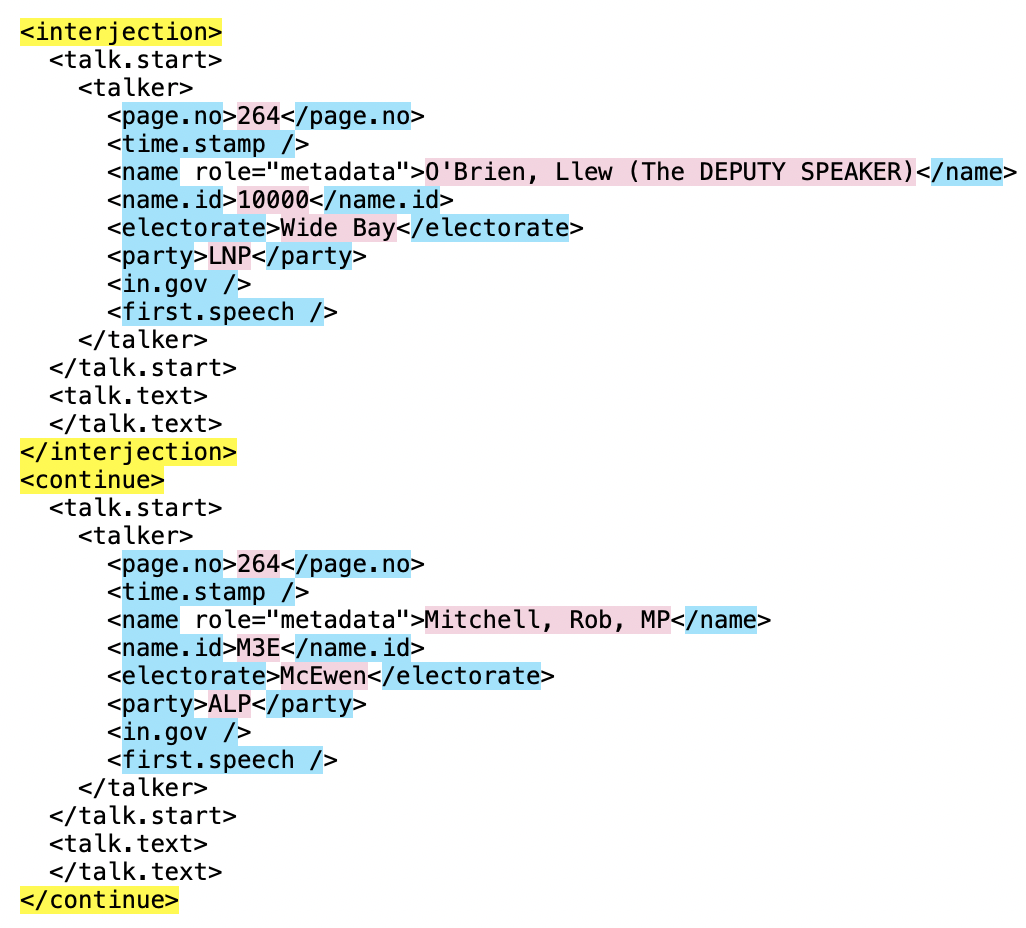
\includegraphics[width=3.59375in,height=\textheight]{xml3.png}

}

\caption{\label{fig-xml3}Snapshot of XML structure with interjection and
continuation from 03 February 2021 Hansard}

\end{figure}

We then created lists using both the \texttt{interject} and
\texttt{main} dataframes to capture all the names of individuals who
spoke that day. We added the names of all Members in a number of unique
formats, due to the frequent variation in how names are transcribed in
Hansard. When a Member interjects or continues a speech, the usual form
of their name is a title followed by their first name or first initial
and/or last name. There is also variation in the capitalization of these
names.\footnote{Sometimes when someones first name is included, only
  their last name is capitalized, while sometimes their full name is
  capitalized, or other times neither are capitalized.} Another source
of variation is in individuals with more than one first name, as
sometimes only their first first name is written, while other times
their entire first name is written. Additionally, some surnames have
punctuation, and some surnames have specific capitalization such as
``McCormack'', where even in full capitalization, the first ``c''
remains lower case. This variation demands careful consideration when
writing regular expression patterns to search for in the text. In these
lists we also accounted for any general interjection statements
transcribed that were not attributed to an individual, such as ``An
opposition member interjecting-''.

Having these lists enabled us to extract the names of Members and their
associated titles as they exist in the text, by searching for exact
matches with regular expression patterns. We then used these extracted
names to split all the speeches up, using a number of regular
expressions with lookarounds. A lookaround can be added to a regular
expression pattern to enhance the specificity of matches. These were
used to ensure that the text was not being split in the wrong places,
such as places where Members were simply being named in the statement of
another Member.

Once all interjections, comments and continuations were successfully
split onto their own rows using the lists we created, we did one final
check for any additional names that were not captured in these lists. To
do so, we searched for any remaining name matches in speech bodies with
general regular expressions and lookarounds, and separated text using
those matches when found.

We then added an order variable to the dataset based on row number, to
keep track of the order in which everything was said. The next step was
to fill the name, name ID, electorate and party variables with the
correct data for each row. We also wanted to add the gender and unique
identifier for each individual as found in the
\texttt{AustralianPoliticians} package. To do so, we created a lookup
table, which contained the unique incomplete form in which the name was
transcribed, and the corresponding full name, name ID, electorate,
party, gender and unique ID for that individual. Figure~\ref{fig-lookup}
provides an example of this. We used the main dataset from the
\texttt{AustralianPoliticians} package in the creation of each lookup
table (Alexander and Hodgetts 2021).

\begin{figure}

{\centering 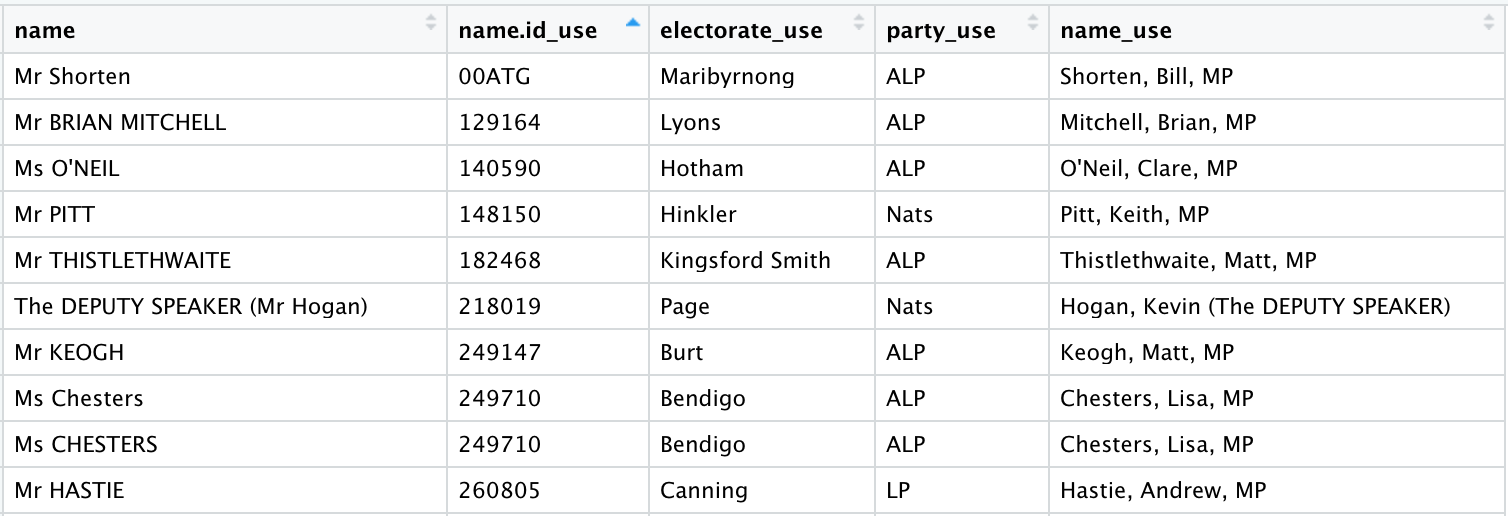
\includegraphics[width=4.66667in,height=\textheight]{lookup_ex.png}

}

\caption{\label{fig-lookup}First 10 rows of lookup table from 19 October
2017 Hansard processing}

\end{figure}

Next, we merged our main dataframe with the lookup table to replace any
incomplete names with their full names, and to fill in any gaps with
available name ID, electorate, party, gender and unique ID information.
Finally, we were able to add a flag for interjections. Grouping our data
by the speech number, we defined an interjection as a statement made by
anyone who is not The Speaker, The Deputy Speaker, or the Member whose
turn it was to speak. Figure~\ref{fig-interject} provides an example of
a Federation Chamber proceeding with interjections. Evidently,
statements made by the original speaker Stuart Robert or by The Deputy
Speaker Maria Vamvakinou are not flagged as interjections.

\begin{figure}

{\centering 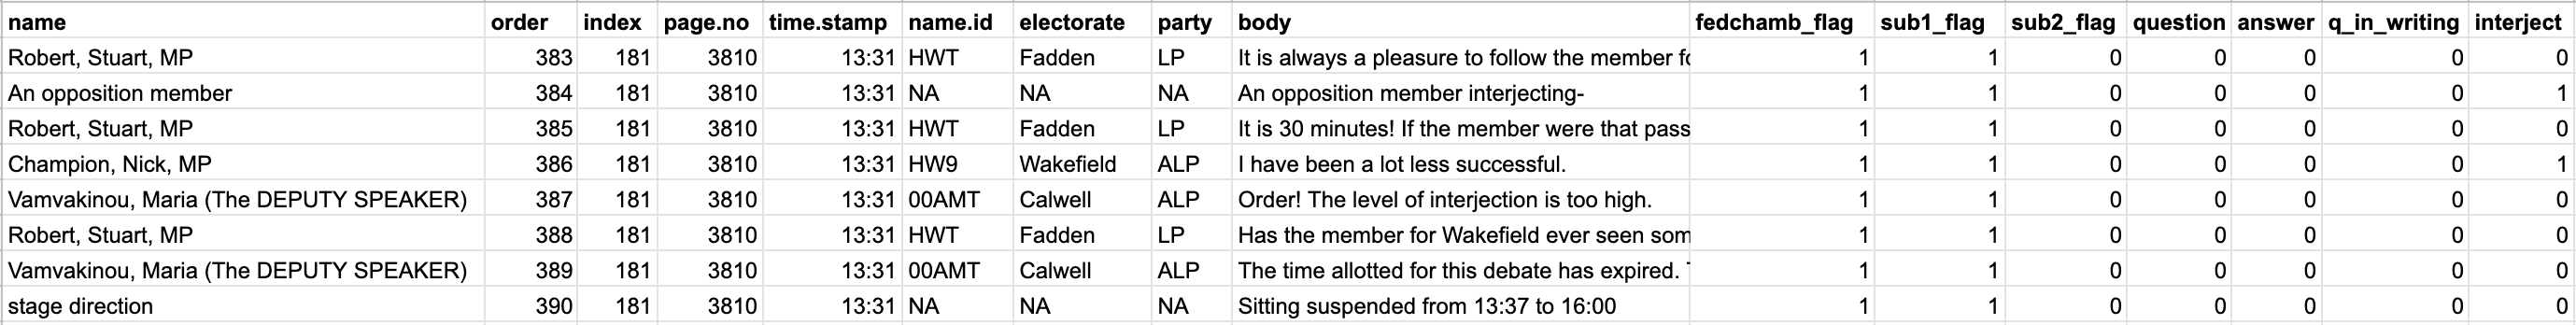
\includegraphics{interject_ex.png}

}

\caption{\label{fig-interject}Example of speech with interjections from
21 November 2016 Hansard}

\end{figure}

Having developed a successful methodology for splitting interjections,
we used this to inform our general approach in the third and fourth
scripts. However, the difference in data cleaning used in these scripts
necessitated some departure from the original methodology. As discussed
in Section~\ref{sec-diff}, we used string patterns extracted from
\texttt{\textless{}talk.start\textgreater{}} nodes to separate speeches.
As evident in Figure~\ref{fig-xml3},
\texttt{\textless{}talk.start\textgreater{}} nodes are nested within
\texttt{\textless{}interjection\textgreater{}} nodes, meaning that the
patterns of data from interjection statements were separated out in the
process. In other words, our approach to data cleaning in the third and
fourth scripts separated out interjections in the process. This meant
that we did not need to create lists of names and titles to search for
in the text as we did before. However, we used the same list of general
interjection statements to separate on that was used in the first two
scripts. We then did an additional check for statements that may have
not been separated due to how they were embedded in the XML, and
separated those out where needed.\footnote{While most statements were
  categorized in their own child-node and hence captured through
  pattern-based separation, some were not individually categorized, and
  had to be split manually in this step.}

We then proceeded to clean up speeches and fill in correct speaker
details. While we used the same lookup table approach as before, we did
so in combination with another means of filling in speaker details. The
patterns parsed from \texttt{\textless{}talk.start\textgreater{}} nodes
contain important data on the speaker of each statement. As such, we
could extract those data associated with each pattern by parsing one
element inward, using the XPath expression
\texttt{\textless{}talk.start/talker\textgreater{}}. We created a
pattern lookup table with these data, and merged it with the main
Hansard dataframe by the first pattern detected in each statement.
Figure~\ref{fig-patterns} provides an example of that lookup table. This
approach enabled us to fill in missing data on each speaker using data
extracted directly from the XML. Finally, we then used the
\texttt{AustralianPoliticians} dataset to fill in other missing data,
and flagged for interjections in the same manner as before.

\begin{figure}

{\centering 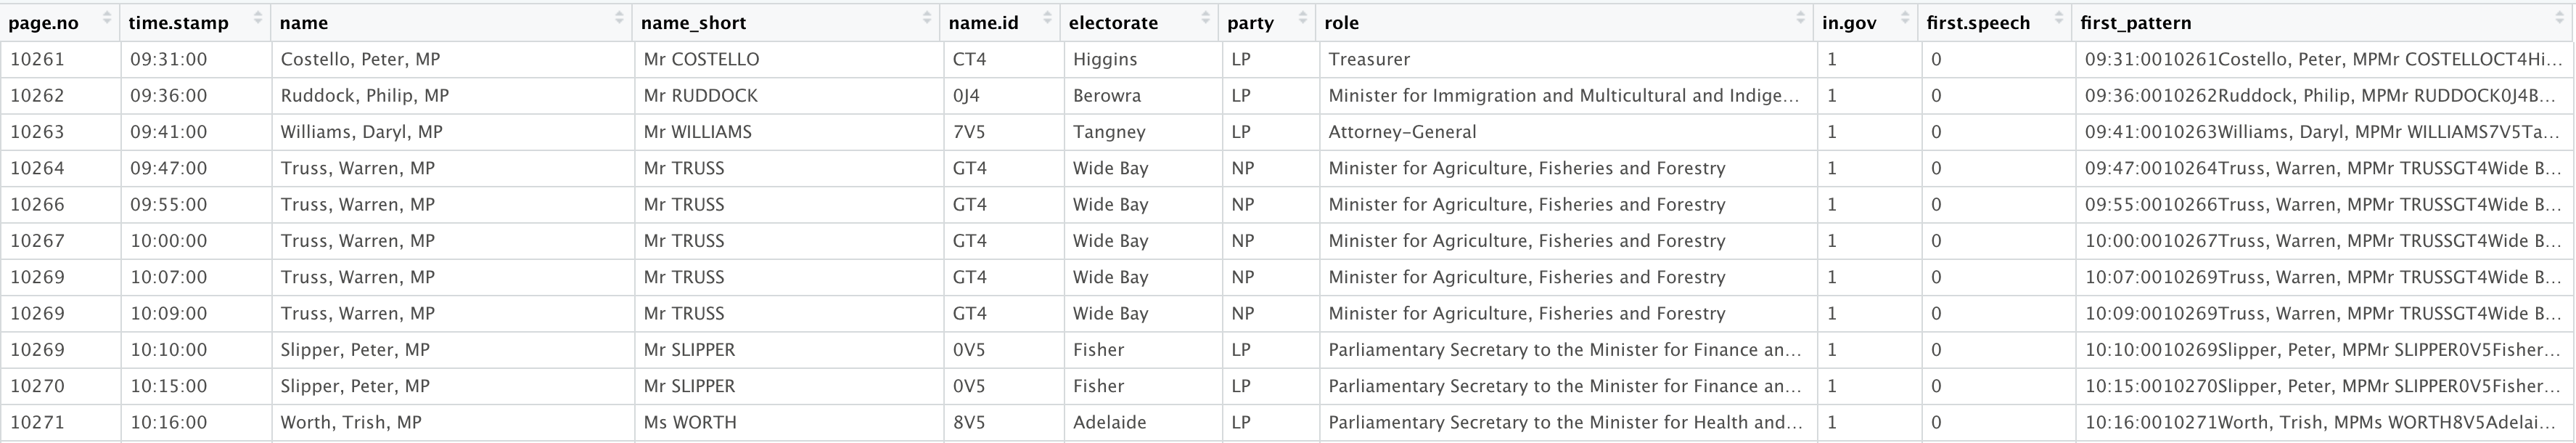
\includegraphics{pattern_lookup.png}

}

\caption{\label{fig-patterns}10 rows of pattern lookup table from 12
December 2012 Hansard processing}

\end{figure}

\hypertarget{sec-stage}{%
\subsection{Stage Directions}\label{sec-stage}}

When building our first scripts, one of the final components needed was
to separate general stage directions out from statements made by
members. Stage directions are general statements included in the
transcript to document happenings in parliament. Examples of stage
directions are ``Bill read a second time'', ``Question agreed to'' or
``Debate adjourned''. It was unclear to us from the XML and PDF who
exactly these statements were attributed to. For further clarification,
we watched portions of the video recording for some sitting days, and
noticed that where these statements are documented in Hansard, they are
not explicitly stated in parliament. For example, when The Deputy
Speaker says ``The question is that the bill be now read a second
time'', members of the House take a vote, and if the majority is in
favour, they proceed reading the bill the second time. This vote and
second reading is not explicitly transcribed, rather what is written is:
``Question agreed to. Bill read a second time''. For this reason, we
filled the name variable for these statements with ``stage direction''.
Note that stage directions were not flagged as interjections. These
stage directions are not defined differently from the regular debate
speech in the XML, meaning we had to manually create a list of stage
directions to separate out of the speeches. We have built this list of
stage directions as we worked backwards in parsing Hansard, and took the
same approach across all four scripts.

\hypertarget{data-records}{%
\section{Data Records}\label{data-records}}

Our database contains 1517 CSV files, covering all sitting days of the
House of Representatives from 02 March 1998 to 08 September 2022. All
data records are available on the general-purpose repository Zenodo, at
https://doi.org/10.5281/zenodo.7336076 (Katz and Alexander 2022). For
each CSV file, each row contains an individual statement, with details
on the individual speaking. Of course, for general statements
transcribed as made by ``Honourable members'' for example, these
variables cannot be specified. Table~\ref{tbl-vars} provides an overview
of each variable found in the database.

\hypertarget{tbl-vars}{}
\begin{table}[H]
\caption{\label{tbl-vars}Summary and description of variables in our database }\tabularnewline

\centering
\begin{tabular}{ll}
\toprule
Variable & Description\\
\midrule
name & Name of speaker\\
order & Row number\\
speech\_no & Speech number\\
page.no & Page number statement can be found on in official Hansard\\
time.stamp & Time of statement\\
\addlinespace
name.id & Unique member identification code, based on the Parliamentary Handbook\\
electorate & Speaking member's electorate\\
party & Speaking member's party\\
in.gov & Flag for in government (1 if in government, 0 otherwise)\\
first.speech & Flag for first speech (1 if first speech, 0 otherwise)\\
\addlinespace
body & Statement text\\
fedchamb\_flag & Flag for Federation Chamber (1 if Federation Chamber, 0 if Chamber)\\
sub1\_flag & Flag for sub-debate 1 contents (1 if sub-debate 1, 0 otherwise)\\
sub2\_flag & Flag for sub-debate 2 contents (1 if sub-debate 2, 0 otherwise)\\
question & Flag for question (1 if question, 0 otherwise)\\
\addlinespace
answer & Flag for answer (1 if answer, 0 otherwise)\\
q\_in\_writing & Flag for question in writing (1 if question in writing, 0 otherwise)\\
div\_flag & Flag for division (1 if division, 0 otherwise)\\
gender & Gender of speaker\\
uniqueID & Unique identifier of speaker\\
\addlinespace
interject & Flag for interjection (1 if statement is an interjection, 0 otherwise)\\
\bottomrule
\end{tabular}
\end{table}

The \texttt{name}, \texttt{page.no}, \texttt{time.stamp},
\texttt{name.id}, \texttt{electorate}, \texttt{party}, \texttt{in.gov},
\texttt{first,speech}, and \texttt{body} variables all came directly
from the XML contents. In addition to these variables, we added a number
of flags to enable easy filtering of statements. For example, adding the
\texttt{fedchamb\_flag} provides a clear distinction between the
proceedings of the Chamber with those of the Federation Chamber. As
well, the \texttt{sub1\_flag} and \texttt{sub2\_flag} variables allow us
to keep track of where various statements are being parsed from in the
XML document. The \texttt{question}, \texttt{answer}, and
\texttt{q\_in\_writing} flags were added to identify statements
belonging to Question Time, and the nature of these statements. We also
flagged for interjections (\texttt{interject}), and the
\texttt{div\_flag} variable was added to flag when a division is called
for. The \texttt{gender} and \texttt{uniqueID} variables were added
based on the main dataset from the \texttt{AustralianPoliticians}
package. Details on the usage of \texttt{uniqueID} will be provided in
Section~\ref{sec-usage}. Further, the \texttt{speech\_no} variable
allows us to keep track of the speech number that each statement and
interjection belongs to. Having the speech number variable offers an
easy way to group statements by speech or isolate specific speeches of
interest. Finally, the \texttt{order} variable was added to maintain the
order of proceedings.

\textbf{this paragraph is a bit repetitive and states everything found
in the table, but i also feel like it's valuable to specify which ones
we added and elaborate on their meaning. thoughts?}

\hypertarget{sec-stats}{%
\subsection{Descriptive Statistics}\label{sec-stats}}

\hypertarget{technical-validation}{%
\section{Technical Validation}\label{technical-validation}}

We developed a script to perform seven automated tests on each file in
our database, in an effort to enhance its quality and consistency. Our
first test validates that the date specified in each file name matches
the date specified in its corresponding XML session header.\footnote{As
  seen in Figure~\ref{fig-xml1}, the first child node of the
  \texttt{\textless{}session.header\textgreater{}} element is the date.}
Every file passed this test, and we detected one discrepancy in an XML
file from 03 June 2009, where its session header contained the wrong
date. We validated that our file name and date was correct by checking
the official PDF release from that sitting day.

The second test checks that in each file, there is an equal number of
flagged questions and answers. This test was motivated by the
discrepancies in correct categorization of questions and answers we
found when parsing Question Time, and allows us to check for the
presence of any of these discrepancies which we have missed.

When a member runs out of allotted time for their speech, Hansard
editors transcribe ``(Time expired)'' after their final word. As a means
of checking that we have separated speeches out correctly, our third
test checks that when the phrase ``(Time expired)'' exists in a body of
text, it exists at the very end. When this is not the case, we know that
we have missed the separation of the next statement onto its own row,
and could fix this accordingly.

The remaining tests focus on the members present on each sitting day.
Our fourth test checks that there is one unique party and electorate
attributed to each individual on each sitting day. As we parsed Hansard
further back in time, we found a number of cases where an individual was
associated with the wrong electorate or party due to transcription
errors. When we found these data errors we corrected them based on the
official release. This test provides us with an automated way to catch
these errors and correct them at scale.

Next, we test that the unique name identification code attributed to
each individual is found in the Australian Parliamentary Handbook. We do
so using the \texttt{ausPH} package. This test serves as another means
to correct for transcription errors, this time in the case of name IDs.
We found and corrected for a number of common name ID transcription
errors detected by this test, such as a capital letter ``O'' in place of
a zero.

Our sixth test checks that on any given sitting day, the individuals
identified are alive. To do so, we utilized the main dataset from the
\texttt{AustralianPoliticians} package which contains the birth and
where applicable death dates for every politician. This test confirmed
that all members who are detected to speak on each sitting day are not
deceased.

Finally, our seventh test validates that all individuals speaking are
active members of parliament on that particular day. We use the
\texttt{mps} dataset from the \texttt{AustralianPoliticians} package
which has the dates of each Member's duration in parliament. Using these
dates, we check that each person speaking on each sitting day is in fact
a Member of Parliament on that day.

\hypertarget{sec-usage}{%
\section{Usage Notes}\label{sec-usage}}

To enhance the usability of our database, we added a \texttt{uniqueID}
variable to each CSV file. This serves as a unique identifier for each
speaking Member, and comes from the \texttt{uniqueID} variable present
within data from both the \texttt{AustralianPoliticians} and
\texttt{AustralianElections} R packages (Alexander and Hodgetts 2021;
Alexander 2019). By including this variable, one can readily integrate
our data records with those available in these two packages.

Further, the \texttt{name.id} variable found in each CSV is another
unique identifier for each Member of Parliament. This variable was
parsed directly from the Hansard XML files, and can be found in the
Australian Parliamentary Handbook. As such, our data records can be
integrated with those from the \texttt{ausPH} package which provides
datasets for contents of the Australian Parliamentary Handbook (Leslie
2021). This will allow for convenient extraction of further details on
each Member of Parliament in a tidy, ready to analyze format.

\hypertarget{code-availability}{%
\section{Code Availability}\label{code-availability}}

The code written to build this database is available on the GitHub
repository associated with this paper:
https://github.com/lindsaykatz/hansard-proj. All scripts were created
using R software (R Core Team 2022). The core packages used to develop
these scripts are: the \texttt{XML} package by Temple Lang (2022), the
\texttt{xml2} package by Wickham, Hester, and Ooms (2021), the
\texttt{tidyverse} R packages by Wickham et al. (2019), the
\texttt{AustralianPoliticians} package by Alexander and Hodgetts (2021),
and the \texttt{ausPH} package by Leslie (2021). \texttt{XML} and
\texttt{xml2} were used for parsing the XML documents,
\texttt{AustralianPoliticians} and \texttt{ausPH} were used for cleaning
up and filling in member details in the datasets, and \texttt{tidyverse}
packages were used in all steps, for tidy wrangling of data.

\hypertarget{acknowledgements}{%
\section{Acknowledgements}\label{acknowledgements}}

\hypertarget{author-contributions}{%
\section{Author Contributions}\label{author-contributions}}

\hypertarget{competing-interests}{%
\section{Competing Interests}\label{competing-interests}}

The authors declare no competing interests.

\hypertarget{references}{%
\section*{References}\label{references}}
\addcontentsline{toc}{section}{References}

\hypertarget{refs}{}
\begin{CSLReferences}{1}{0}
\leavevmode\vadjust pre{\hypertarget{ref-auselect}{}}%
Alexander, Rohan. 2019. \emph{AustralianElections: Datasets on
Australian Elections}.
\url{https://github.com/RohanAlexander/AustralianElections}.

\leavevmode\vadjust pre{\hypertarget{ref-alexander2021}{}}%
Alexander, Rohan, and Monica Alexander. 2021. {``The Increased Effect of
Elections and Changing Prime Ministers on Topics Discussed in the
Australian Federal Parliament Between 1901 and 2018.''} \emph{arXiv
Preprint arXiv:2111.09299}.

\leavevmode\vadjust pre{\hypertarget{ref-auspol}{}}%
Alexander, Rohan, and Paul A. Hodgetts. 2021.
\emph{AustralianPoliticians: Provides Datasets about Australian
Politicians}.
\url{https://CRAN.R-project.org/package=AustralianPoliticians}.

\leavevmode\vadjust pre{\hypertarget{ref-lipad}{}}%
Beelen, Kaspar, Timothy Alberdingk Thijm, Christopher Cochrane, Kees
Halvemaan, Graeme Hirst, Michael Kimmins, Sander Lijbrink, et al. 2017.
{``Digitization of the Canadian Parliamentary Debates.''} \emph{Canadian
Journal of Political Science/Revue Canadienne de Science Politique} 50
(3): 849--64.

\leavevmode\vadjust pre{\hypertarget{ref-fraussen2018}{}}%
Fraussen, Bert, Timothy Graham, and Darren R Halpin. 2018. {``Assessing
the Prominence of Interest Groups in Parliament: A Supervised Machine
Learning Approach.''} \emph{The Journal of Legislative Studies} 24 (4):
450--74.

\leavevmode\vadjust pre{\hypertarget{ref-australia2018house}{}}%
House of Representatives. 2018. Edited by D. R. Elder and P. E. Fowler.
\emph{{House of Representatives Practice}}. 7th ed. {Australian
Government - Department of the House of Representatives}.

\leavevmode\vadjust pre{\hypertarget{ref-house2021}{}}%
---------. 2021. \emph{{A window on the house: Practices and procedures
relating to question time}}. {Parliament of Australia}.

\leavevmode\vadjust pre{\hypertarget{ref-katz_2022}{}}%
Katz, Lindsay, and Rohan Alexander. 2022. {``{A new, comprehensive
database of all proceedings of the Australian Parliamentary Debates}.''}
Zenodo. \url{https://doi.org/10.5281/zenodo.7336076}.

\leavevmode\vadjust pre{\hypertarget{ref-Leslie_2021_HoR_Aus}{}}%
Leslie, Patrick. 2021. \emph{Members of the Australian House of
Representatives (1945-2019)}.
\url{https://github.com/palesl/AustralianHouseOfRepresentatives}.

\leavevmode\vadjust pre{\hypertarget{ref-r_software}{}}%
R Core Team. 2022. \emph{R: A Language and Environment for Statistical
Computing}. Vienna, Austria: R Foundation for Statistical Computing.
\url{https://www.R-project.org/}.

\leavevmode\vadjust pre{\hypertarget{ref-rasiah2010framework}{}}%
Rasiah, Parameswary. 2010. {``A Framework for the Systematic Analysis of
Evasion in Parliamentary Discourse.''} \emph{Journal of Pragmatics} 42
(3): 664--80.

\leavevmode\vadjust pre{\hypertarget{ref-salisbury2011}{}}%
Salisbury, Christopher. 2011. {``'Mr Speaker, i Withdraw...': Standards
of (Mis) Behaviour in the Queensland, Western Australian and
Commonwealth Parliaments Compared via Online Hansard.''}
\emph{Australasian Parliamentary Review} 26 (1): 166--77.

\leavevmode\vadjust pre{\hypertarget{ref-sherratt}{}}%
Sherratt, Tim. 2016. {``Documentation: Historic Hansard.''}
\emph{Historic Hansard}.
\url{http://timsherratt.org/digital-heritage-handbook/docs/historic-hansard/\#}.

\leavevmode\vadjust pre{\hypertarget{ref-XML_pkg}{}}%
Temple Lang, Duncan. 2022. \emph{XML: Tools for Parsing and Generating
XML Within r and s-Plus}. \url{https://CRAN.R-project.org/package=XML}.

\leavevmode\vadjust pre{\hypertarget{ref-vice2017history}{}}%
Vice, John, and Stephen Farrell. 2017. \emph{The History of Hansard}.
House of Lords Library; House of Lords Hansard.

\leavevmode\vadjust pre{\hypertarget{ref-tidyverse}{}}%
Wickham, Hadley, Mara Averick, Jennifer Bryan, Winston Chang, Lucy
D'Agostino McGowan, Romain François, Garrett Grolemund, et al. 2019.
{``Welcome to the {tidyverse}.''} \emph{Journal of Open Source Software}
4 (43): 1686. \url{https://doi.org/10.21105/joss.01686}.

\leavevmode\vadjust pre{\hypertarget{ref-xml2_pkg}{}}%
Wickham, Hadley, Jim Hester, and Jeroen Ooms. 2021. \emph{Xml2: Parse
XML}. \url{https://CRAN.R-project.org/package=xml2}.

\end{CSLReferences}



\end{document}
